Bei den beiden Convolution Direct Cascade Netzwerken ist der einzige Unterschied, dass sie die Bilder in ein- beziehungsweise in 
zweidimensionaler Form sehen. Dabei fällt aber auf, dass es im zweidimensionalen Fall etwas besser ist. 
Dies liegt daran, dass das eindimensionale Netz in dem Filterlayer nur die Daten direkt rechts und links mit einbezieht. Das 
zweidimensionale Netzwerk hingegen nutzt bei der Operation jenes Layers nicht nur die direkt rechts und links, sondern auch die Daten, 
die oben und unten angrenzend sind, sowie die Daten, die in jede Richtung schräg vorkommen. 
Die Verbesserung ist aber nur minimal, wie in Figure 4.3 zu sehen. 

\begin{figure}[htpb]
    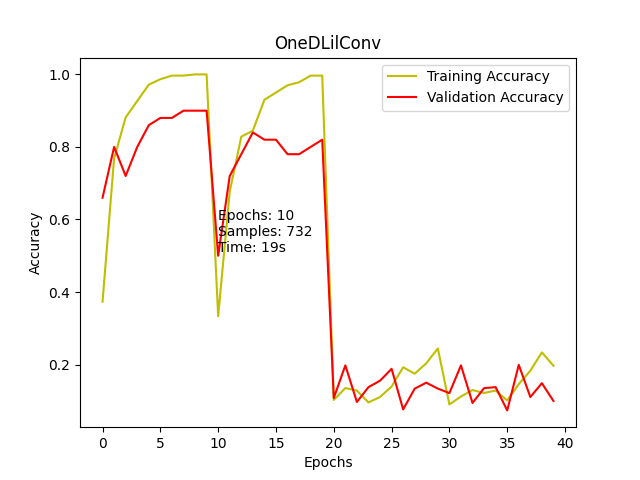
\includegraphics[height=5cm]{../../Plots/ba_plots/dimensionality/1dim_tr.png}
    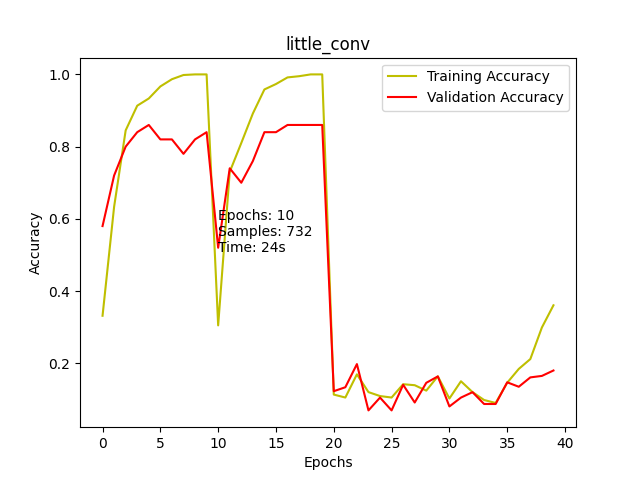
\includegraphics[height=5cm]{../../Plots/ba_plots/dimensionality/2dim_tr.png}
    \caption{\label{fig:dim} Vergleich 1D mit 2D}
\end{figure}

Da das zweidimensionale Netzwerk mit nicht so vielen Daten genutzt werden kann, hat es hier eine sehr viel kürzere Zeit. Es kann deshalb 
nicht genutzt werden, da die Berechnung des Augmented Vectors zu Speicherplatzproblemen im Arbeitsspeicher führt. 

Weil diese Veränderung nur minimal ist, reicht es nur das eindimensionale Netz in den meisten Fällen zu betrachten, weshalb die technischen 
Probleme beim zweidimensionalen Netzwerk nicht so hinderlich für die Evaluierung von TF sind. 
